\chapter{光与影}\label{ch:g1:light-and-shadows}

关掉没有窗户的房间里的灯：一切都不见了。
打开灯：房间又回来了。看见东西需要光。
只要有光，就有\omterm{def:g1:light-and-shadows:shadow}{影子}——你忠实的黑色“孪生兄弟”
总是跟着你走过每一块晴天的人行道。让我们来看看光从哪里来，
以及\omterm{def:g1:light-and-shadows:shadow}{影子}是怎样形成的。

\section{光从哪里来}

\begin{definition}[光源]\label{def:g1:light-and-shadows:source}
自己能发光的东西称为\emph{光源}\index{光源}，
即自身发出的\emph{光}\index{光}，如太阳、电灯、
蜡烛火焰和萤火虫。其他东西——书、球、墙壁和你——都不发光，
我们只有在光源发出的光照到它们上面时，
才能看见它们。
\end{definition}

\begin{example}[是不是光源？]\label{ex:g1:light-and-shadows:sources}
太阳、手电筒、燃着的火柴和电视屏幕都会发光，它们都是\omterm{def:g1:light-and-shadows:source}{光源}。
月球、镜子和白墙看起来可以很亮，
但它们自己并不发光，只是把照到它们身上的光
反射回来。关掉灯，
最亮的镜子也会变暗。
\end{example}

\begin{example}[动手试一试：黑暗的房间]\label{ex:g1:light-and-shadows:darkroom}
傍晚时，把房间的百叶窗或窗帘拉上，
关掉每一盏灯，慢慢数到 $20$，你看到了什么？
起初几乎什么也看不见——没有\omterm{def:g1:light-and-shadows:source}{光源}，就没有光让我们看东西。
然后把门开一条缝：一线细细的光
就足以让桌子、椅子和玩具重新出现。
\end{example}

\begin{remark}[永远不要直视太阳]\label{rem:g1:light-and-shadows:sun}
太阳是我们见过的最强\omterm{def:g1:light-and-shadows:source}{光源}。千万不要直视它，
哪怕只看一瞬间，也不要透过双筒望远镜或放大镜去看，
它的光非常强，会永久伤害你的眼睛。
太阳应当从侧面欣赏——
欣赏它照亮其他一切事物的光。
\end{remark}

\section{影子是怎样形成的}

\begin{definition}[影子]\label{def:g1:light-and-shadows:shadow}
挡住光的物体后面出现的暗斑称为\emph{影子}\index{影子}。
光无法穿过你的身体，因此你身后的地面
得不到太阳的光，
那块像你形状的暗斑就是你的影子。
\end{definition}

\begin{omfigure}
\begin{tikzpicture}[scale=0.85]
  % two rays from the lamp, exactly tangent to the ball (computed:
  % source (0,1.5), ball center (4.2,1.5), r=0.55 -> wall hits y=1.5±1.004)
  \draw[omThm] (0,1.5) -- (7.6,2.504);
  \draw[omThm] (0,1.5) -- (7.6,0.496);
  % free rays that miss the ball entirely
  \draw[omThm] (0,1.5) ++(32:0.42) -- ++(32:2.4);
  \draw[omThm] (0,1.5) ++(-32:0.42) -- ++(-32:2.4);
  \fill[omThm] (0,1.5) circle (0.3);
  \draw[thick, fill=omDef, fill opacity=0.3] (4.2,1.5) circle (0.55);
  \draw[very thick] (7.6,-0.4) -- (7.6,3.4);
  \draw[line width=3.5pt, omExo] (7.6,0.496) -- (7.6,2.504);
  \node[below, font=\small] at (0,1.0) {灯};
  \node[below, font=\small] at (4.2,0.7) {球};
  \node[right, font=\small] at (7.75,1.5) {影子};
  \node[right, font=\small] at (7.75,3.0) {墙};
\end{tikzpicture}

{\small 灯发光，球挡住了光，身后的墙保持暗色：
灯、挡光的物体、\omterm{def:g1:light-and-shadows:shadow}{影子}——总是按这个顺序，排成一条直线。}
\end{omfigure}

\begin{method}[做出清晰的影子]\label{met:g1:light-and-shadows:make}
\begin{enumerate}
  \item 把房间弄暗——
        光从各处照来时，\omterm{def:g1:light-and-shadows:shadow}{影子}就会隐藏起来；
  \item 打开\emph{一}盏灯或手电筒；
  \item 把玩具拿在灯和墙之间；
  \item 看墙面：\omterm{def:g1:light-and-shadows:shadow}{影子}就在玩具
        背离灯的那一侧。
\end{enumerate}
把玩具靠近灯：\omterm{def:g1:light-and-shadows:shadow}{影子}变得非常大。
把玩具靠近墙：\omterm{def:g1:light-and-shadows:shadow}{影子}缩小到玩具的真实大小。
\end{method}

\begin{example}[动手试一试：影子动物]\label{ex:g1:light-and-shadows:animals}
用\cref{met:g1:light-and-shadows:make}中的灯，不用玩具，
把双手放进光里：两根手指竖起，做成兔子耳朵；
两只大拇指交叉，做成一只飞鸟。墙上显示的是
你的手在光中挡出的形状——\omterm{def:g1:light-and-shadows:shadow}{影子}总是保持
从灯的方向看去，挡光物的形状。
\end{example}

\begin{remark}[影子不是实物]\label{rem:g1:light-and-shadows:notathing}
你不能捡起\omterm{def:g1:light-and-shadows:shadow}{影子}，不能折叠它，也不能把它装进盒子。\omterm{def:g1:light-and-shadows:shadow}{影子}
不是由任何东西构成的，它是一处\emph{光线缺失的地方}——
这就是灯一熄灭\omterm{def:g1:light-and-shadows:shadow}{影子}就消失的原因——
那里没有任何东西能留下来。
\end{remark}

\section{影子随光而定}

\begin{example}[影子在哪一侧？]\label{ex:g1:light-and-shadows:opposite}
早晨，太阳在你的一边，
\omterm{def:g1:light-and-shadows:shadow}{影子}则落在\emph{另一边}。面向太阳，\omterm{def:g1:light-and-shadows:shadow}{影子}藏在你身后。
背对太阳，\omterm{def:g1:light-and-shadows:shadow}{影子}就伸到你的前方。
\omterm{def:g1:light-and-shadows:shadow}{影子}总是正好位于\omterm{def:g1:light-and-shadows:source}{光源}的对面。
\end{example}

\begin{omfigure}
\begin{tikzpicture}[scale=0.75]
  % low sun: the ray from the Sun grazing the stick's tip is drawn
  % straight; the shadow ends exactly where that ray meets the ground
  % (sun (0.7,2.2), tip (3.4,1.2) -> ground at x=6.64)
  \fill[omThm] (0.7,2.2) circle (0.4);
  \foreach \a in {0,45,...,315} {
    \draw[omThm] (0.7,2.2) ++(\a:0.55) -- ++(\a:0.25);
  }
  \draw[omThm] (0.7,2.2) -- (6.64,0);
  \draw[line width=2.6pt] (3.4,0) -- (3.4,1.2);
  \draw[thick] (2.2,0) -- (7.0,0);
  \draw[line width=3.5pt, omExo] (3.4,-0.09) -- (6.64,-0.09);
  \node[below, font=\small] at (4.6,-0.35) {太阳低：影子长};
  % high sun: same stick, the grazing ray is steep
  % (sun (8.6,3.6), tip (10.2,1.2) -> ground at x=11.0)
  \fill[omThm] (8.6,3.6) circle (0.4);
  \foreach \a in {0,45,...,315} {
    \draw[omThm] (8.6,3.6) ++(\a:0.55) -- ++(\a:0.25);
  }
  \draw[omThm] (8.6,3.6) -- (11.0,0);
  \draw[line width=2.6pt] (10.2,0) -- (10.2,1.2);
  \draw[thick] (9.0,0) -- (11.8,0);
  \draw[line width=3.5pt, omExo] (10.2,-0.09) -- (11.0,-0.09);
  \node[below, font=\small] at (10.4,-0.35) {太阳高：影子短};
\end{tikzpicture}

{\small 同一根木棍，分别在早晨和中午。\omterm{def:g1:light-and-shadows:shadow}{影子}的末端
正好落在贴着木棍顶端的那条直线光线与
地面相交的地方：低太阳把\omterm{def:g1:light-and-shadows:shadow}{影子}拉得很长，高太阳使\omterm{def:g1:light-and-shadows:shadow}{影子}变短。}
\end{omfigure}

\begin{omfigure}
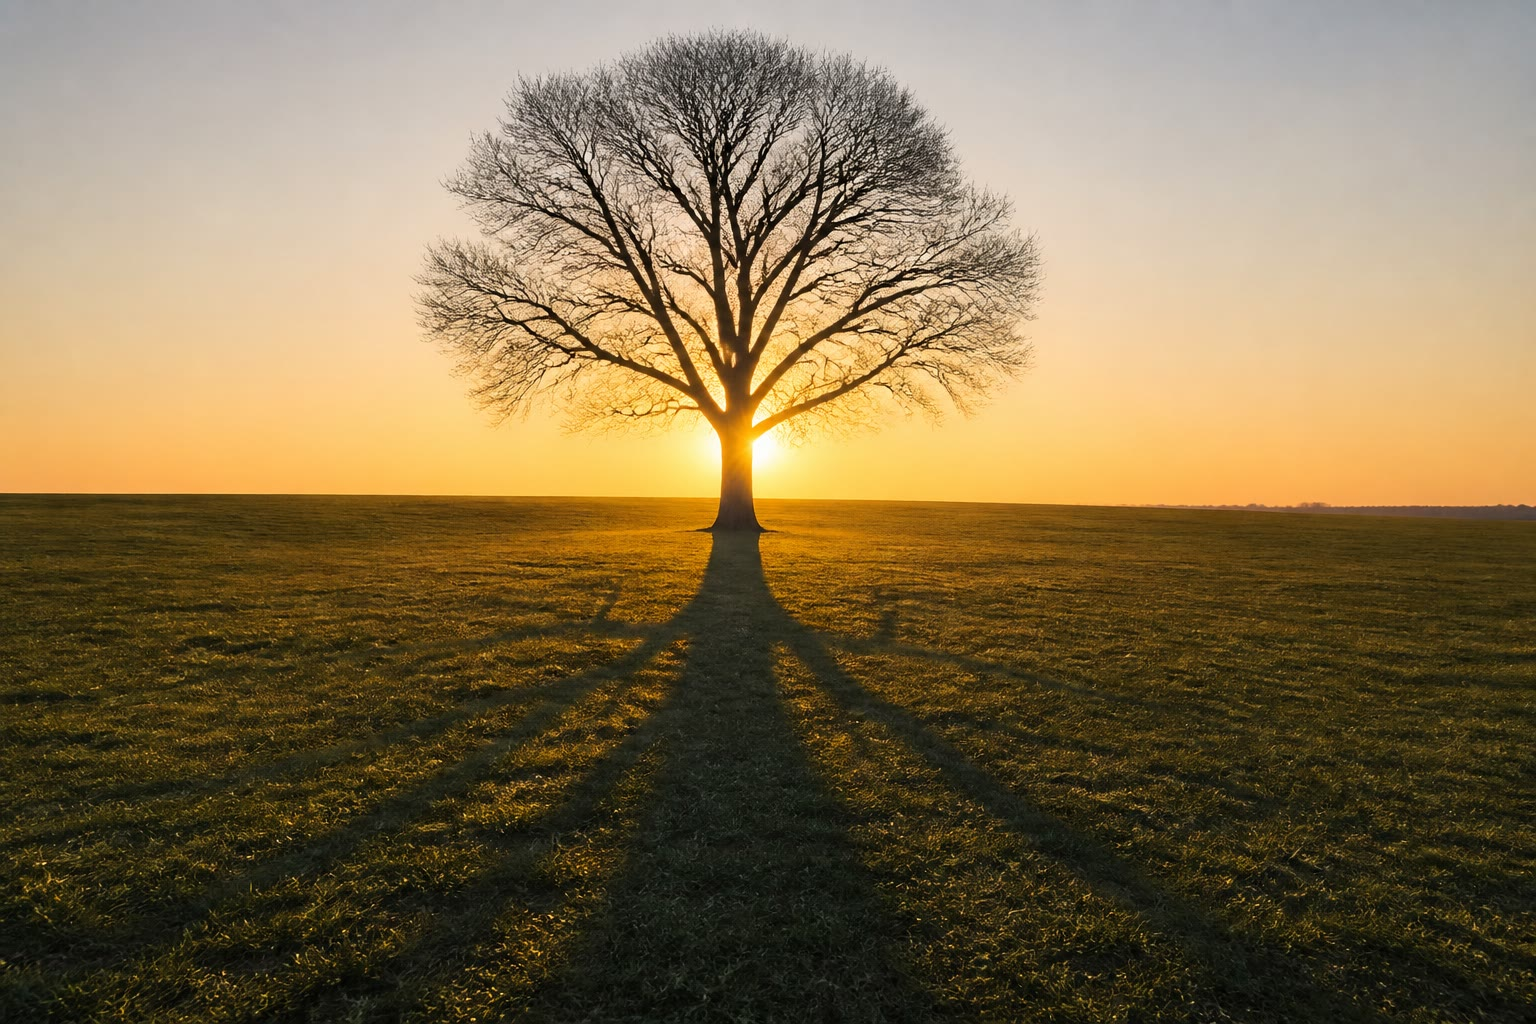
\includegraphics[width=0.6\linewidth]{images/book1/ai/g1-light-shadows-long-shadow.jpg}

{\small 傍晚时太阳低挂，\omterm{def:g1:light-and-shadows:shadow}{影子}很长：太阳越低，每个\omterm{def:g1:light-and-shadows:shadow}{影子}伸得越远。}
\end{omfigure}

\begin{example}[试一试：用粉笔画影子]\label{ex:g1:light-and-shadows:chalk}
在一个晴朗的早晨，站在操场上一动不动，让朋友
用粉笔沿你的\omterm{def:g1:light-and-shadows:shadow}{影子}画一圈。午饭后回到同一位置站好，
你会发现\omterm{def:g1:light-and-shadows:shadow}{影子}已经移出了粉笔线，
而且长度也变了！太阳在天空中换了位置——
\omterm{def:g1:light-and-shadows:shadow}{影子}也跟着变了。下一章将跟随太阳走过
它的一整天。
\end{example}

\section{练习}

\begin{exercise}[$\star$]\label{exo:g1:light-and-shadows:1}
把下列物体分为\omterm{def:g1:light-and-shadows:source}{光源}和非\omterm{def:g1:light-and-shadows:source}{光源}：烛焰；\ 月球；
\ 萤火虫；\ 镜子；\ 手电筒；\ 白墙。
\end{exercise}

\begin{exercise}[$\star$]\label{exo:g1:light-and-shadows:2}
为什么在一间没有窗户、也没有灯的封闭房间里，
你什么也看不见？缺少的是什么？
\end{exercise}

\begin{exercise}[$\star$]\label{exo:g1:light-and-shadows:3}
说出在墙上形成\omterm{def:g1:light-and-shadows:shadow}{影子}所需的三样东西，
并把它们按正确顺序排成一条直线。
\end{exercise}

\begin{exercise}[$\star$]\label{exo:g1:light-and-shadows:4}
太阳在你的左边，你的\omterm{def:g1:light-and-shadows:shadow}{影子}在哪一侧？你转过身来，
整个转身之后，\omterm{def:g1:light-and-shadows:shadow}{影子}在哪里？
\end{exercise}

\begin{exercise}[$\star$]\label{exo:g1:light-and-shadows:5}
利用\cref{met:g1:light-and-shadows:make}，用同一个玩具先做出
很大的\omterm{def:g1:light-and-shadows:shadow}{影子}，再做出很小的\omterm{def:g1:light-and-shadows:shadow}{影子}。你移动了什么？向哪个方向移动？
\end{exercise}

\begin{exercise}[$\star$]\label{exo:g1:light-and-shadows:6}
\omterm{def:g1:light-and-shadows:shadow}{影子}能被捡起来放进口袋吗？请说明\omterm{def:g1:light-and-shadows:shadow}{影子}究竟是什么，
并利用\cref{rem:g1:light-and-shadows:notathing}作答。
\end{exercise}

\begin{exercise}[$\star$]\label{exo:g1:light-and-shadows:7}
为什么绝对不能直视太阳，即使看灯
只会让人有点刺眼？
\end{exercise}

\begin{exercise}[$\star$]\label{exo:g1:light-and-shadows:8}
中午太阳高挂；傍晚时太阳低垂。
什么时候你的\omterm{def:g1:light-and-shadows:shadow}{影子}更长？画出一棵树的两个\omterm{def:g1:light-and-shadows:shadow}{影子}，
分别对应两个时刻。
\end{exercise}

\begin{exercise}[$\star\star$]\label{exo:g1:light-and-shadows:9}
米娅说：“我的\omterm{def:g1:light-and-shadows:shadow}{影子}原来在我前面，我转身之后，
\omterm{def:g1:light-and-shadows:shadow}{影子}就跑到了我身后——所以\omterm{def:g1:light-and-shadows:shadow}{影子}随我一起转动了。”萨姆则说，
\omterm{def:g1:light-and-shadows:shadow}{影子}其实从来没有动过。结合
\cref{ex:g1:light-and-shadows:opposite}想一想：谁说得对？为什么\omterm{def:g1:light-and-shadows:shadow}{影子}
\emph{看起来}像是转动了？
\end{exercise}
